\documentclass[10pt,a4paper]{article}
\usepackage[utf8]{inputenc}
\usepackage{amsmath}
\usepackage{amsfonts}
\usepackage{amssymb}
\usepackage{graphicx}
\title{Soil Carbon Models}
\date{11/21/2016}
\begin{document}
\maketitle
\section*{Century Model}
The flow diagram for the century model proposed by Parton et al. (1988) is shown in Figure 1. In this document, we re-write the model in terms of a set of differential equations. In this model, we have 5 pools, each with a different turnover times: 
\begin{itemize}
\item[pool 1:] \makebox[2.5cm]{Structural C,\hfill}  $\kappa_1 \approx 1/3$,
\item[pool 2:] \makebox[2.5cm]{Metabolic C,\hfill} $\kappa_2 \approx 1/0.5$,
\item[pool 3:] \makebox[2.5cm]{Active Soil C,\hfill}  $\kappa_3 \approx 1/1.5$,
\item[pool 4:] \makebox[2.5cm]{Slow Soil C,\hfill} $\kappa_4 \approx 1/25$,
\item[pool 5:] \makebox[2.5cm]{Passive Soil C,\hfill}  $\kappa_5 \approx 1/1000$,
\end{itemize}
where $\kappa$ denotes the decay rate which is defined as 1 over the turnover. 

We denote the transfer rate from pool $j$ to pool $i$ by $r_{ij}$. The transfer rates are parameterized as a ratio of the decay rate: $r_{ij} = \alpha_{ij} \kappa_j$. From Figure 1, we have:
\begin{align*}
\alpha_{31} & =  (1-\text{A})(1-0.45 \times \text{SL} - 0.55 \times \text{BL}), \\
\alpha_{41} & =  0.7 \times \text{A}, \\
\alpha_{32} & = 0.45, \\
\alpha_{43} & = 1 - F(\text{T}) - 0.004, \\
\alpha_{53} & = 0.004, \\
\alpha_{34} & = 0.42, \\
\alpha_{54} & = 0.03, \\
\alpha_{35} & = 0.45,
\end{align*}
where `SL' is the surface litter, `BL' is the soil litter, `A' is the Lignin fraction, `T' is the soil silt + clay content, and $F(\text{T}) = 0.85 - 0.68 \times \text{T}$. The rest of the transfer coefficients are zero. 

For each pool, we can write the following differential equation:
\begin{equation*}
\frac{d C_i(t)}{dt} = I_i(t) -\kappa_i C_i(t) + \sum_{j\neq i} \alpha_{ij} \kappa_j,
\end{equation*}
where $I_i(t)$ is the external input flow to pool $i$. As far as I understand, in the century model, the input flows are due to the plant residues and only enter the first two pools. Denoting the total flow due to plant residue by $I$, we have:
\begin{align*}
I_1(t) & = (1-\text{L/N})\times I, \\
I_2(t) & = \text{L/N}\times I,
\end{align*}
where L/N denotes the Lignin to Nitrogen ratio. Combining all these differential equations into a single formula, we get:
\begin{equation*}
\frac{dC(t)}{dt} = \left( {\begin{array}{c}
   (1-\text{L/N})\times I \\ \text{L/N}\times I \\ 0   \\ 0 \\ 0  \end{array} } \right) + 
   \left( {\begin{array}{ccccc}
   -\kappa_1 & 0 & 0 & 0 & 0 \\       
   0 & -\kappa_2 & 0 & 0 & 0 \\ 
   \alpha_{31}\kappa_1 & \alpha_{32}\kappa_2 & -\kappa_3 & \alpha_{34}\kappa_4 & \alpha_{35}\kappa_5 \\
   \alpha_{41}\kappa_1 & 0 & \alpha_{43}\kappa_3 & -\kappa_4& 0  \\
   0 & 0 & \alpha_{53}\kappa_3 & \alpha_{54}\kappa_4 & -\kappa_5    
   \end{array} } \right) C(t).
\end{equation*}
\begin{figure}[!h]
\centering
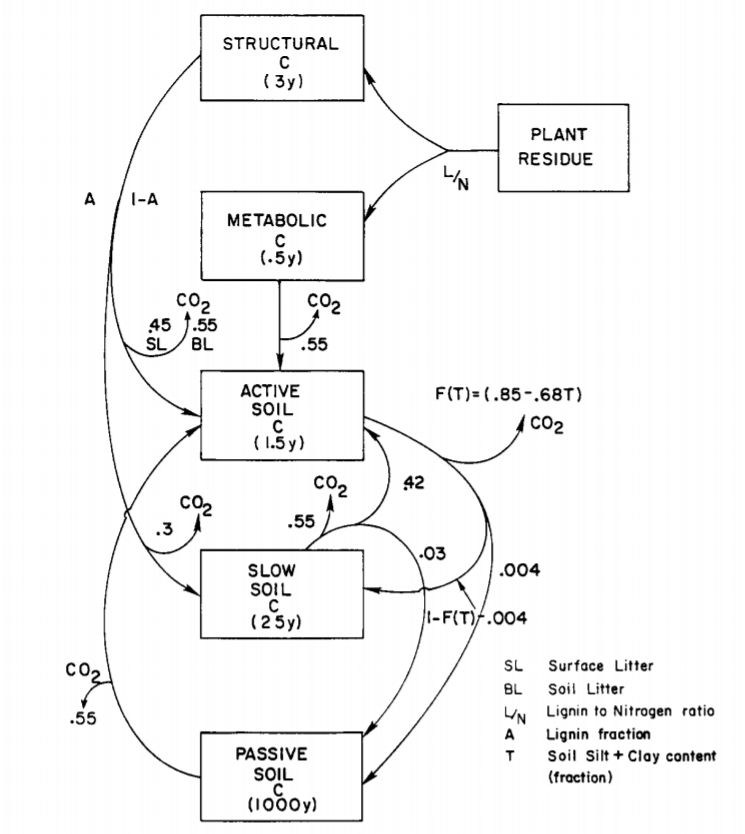
\includegraphics[scale=0.85]{century}
\caption{Flow diagram of century model}
\end{figure}


\section*{CN Model}
The flow diagram of the CN model, developed by Thronton et al., is shown in Figure 2. There are six pools:
\begin{itemize}
\item[pool 1:] \makebox[1.5cm]{Lit1,\hfill}  $\kappa_1 \approx 0.7$,
\item[pool 2:] \makebox[1.5cm]{Lit2,\hfill} $\kappa_2 \approx 0.07$,
\item[pool 3:] \makebox[1.5cm]{Lit3,\hfill}  $\kappa_3 \approx 0.014$,
\item[pool 4:] \makebox[1.5cm]{SOM1,\hfill} $\kappa_4 \approx 0.07$,
\item[pool 5:] \makebox[1.5cm]{SOM2,\hfill}  $\kappa_5 \approx 0.014$,
\item[pool 6:] \makebox[1.5cm]{SOM3,\hfill}  $\kappa_6 \approx 0.0005$.
\end{itemize}
The transfer rate coefficients are:
\begin{equation*}
\alpha_{41}  = 0.61, \quad \alpha_{52}  = 0.45, \quad \alpha_{63}  = 0.71, \quad \alpha_{54} = 0.72, \quad \alpha_{65} = 0.56.
\end{equation*}
So,
\begin{equation*}
\frac{dC(t)}{dt} = \left( {\begin{array}{c}
    I_1 \\ I_2 \\ I_3   \\ 0 \\ 0  \\ 0 \end{array} } \right) + 
   \left( {\begin{array}{cccccc}
   -\kappa_1 & 0 & 0 & 0 & 0 & 0\\       
   0 & -\kappa_2 & 0 & 0 & 0 & 0\\ 
   0 & 0 & -\kappa_3 & 0 & 0 & 0 \\
   \alpha_{41}\kappa_1 & 0 & 0 & -\kappa_4 & 0 & 0 \\
   0 &  \alpha_{52}\kappa_2 & 0 & \alpha_{54}\kappa_4 & -\kappa_5 & 0 \\
   0 & 0 & \alpha_{63}\kappa_3 & 0 & \alpha_{65}\kappa_5 & -\kappa_6    
   \end{array} } \right) C(t).
\end{equation*}
\begin{figure}[!h]
\centering
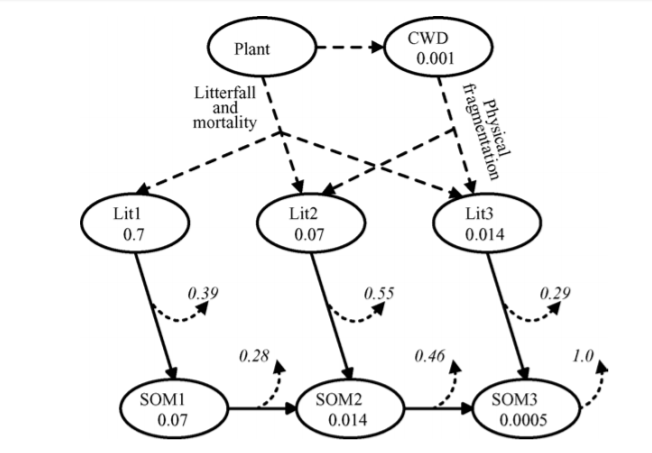
\includegraphics[scale=0.9]{cn}
\caption{Flow diagram of CN model}
\end{figure}
\end{document}